\documentclass[autodetect-engine,dvipdfmx-if-dvi,ja=standard,a4j,jbase=10.5pt,twoside,twocolumn,magstyle=nomag*]{bxjsarticle}
% \documentclass[uplatex, dvipdfmx, a4j, 10ptj, twoside, twocolumn]{jsarticle}
% small japanese font size:     9pt, 10pt, 11pt, 12pt, 14pt, ... (please refer the document of jsclasses)
% word-like japanese font size: 10ptj 10.5ptj, 11ptj, 12ptj (or jbase=xxpt (without 'j') if error is occured)

\usepackage{ifptex,ifxetex,ifluatex}
\ifluatex
    \usepackage{bxcalcux}
    \ltjsetparameter{jacharrange={-2,-3}}
    \usepackage{luatexja-otf}
    \usepackage{bxbase}
\else\ifxetex
    % \usepackage{zxjatype}
    % \usepackage[macros]{zxotf}
    \XeTeXgenerateactualtext=1
    \usepackage{xltxtra}
    \usepackage{bxbase}
\else\ifuptex
    \usepackage{otf}
    \usepackage[prefernoncjk]{pxcjkcat}
    \cjkcategory{sym11,sym18,sym19}{cjk}
    \usepackage[utf8]{inputenc}
    \usepackage{pxbase}
\else\ifstrictptex
    \usepackage{otf}
    \usepackage[utf8]{inputenc}
    \usepackage{pxbase}
\fi\fi\fi\fi

\usepackage[LGR,T2A,T1]{fontenc}

\usepackage{graphicx}
% \usepackage[dvipdfmx]{graphicx}
\usepackage{grffile}

% paper layout setting
\setpagelayout{noheadfoot, left=18.0truemm, right=18.0truemm, top=29.0truemm, bottom=26.0truemm, columnsep=6.5truemm}
% \setpagelayout{noheadfoot, left=15.0truemm, right=5.0truemm, top=12.5truemm, bottom=12.5truemm, columnsep=5.0truemm}

% font setting
\usepackage{amsmath}
\usepackage{amssymb}
\usepackage{mathtools}
\usepackage{bm}
\usepackage{fix-cm}
\usepackage{newtxtext}
\usepackage[slantedGreek]{newtxmath}

% caption setting
\usepackage[font=bf,labelfont=bf,labelsep=quad]{caption}

% to balance the last page of the two-column article
% \usepackage[nospread, keeplastbox, nodebug]{flushend}

% title font style
\renewcommand{\headfont}{\bfseries}

% section setting (using titlesec, uelm package)
\renewcommand{\thesection}{\arabic{section}}
\renewcommand{\thesubsection}{\arabic{section}.\arabic{subsection}}

\usepackage[explicit]{titlesec}
\usepackage[normalem]{ulem}
\titleformat{name=\section}{\normalfont\headfont\normalsize\raggedright}{}{0pt}{\uline{\thesection.\quad#1}}
\titleformat{name=\section,numberless}{\normalfont\headfont\normalsize\raggedright}{}{0pt}{\uline{#1}}
% \titleformat{name=\section}{\normalfont\headfont\normalsize\raggedright}{}{0pt}{\thesection.\quad#1}
\titlespacing{name=\section}{0pt}{.5\Cvs plus .0\Cvs minus .3\Cvs}{.1\Cvs plus .0\Cvs minus .1\Cvs}
\titleformat{name=\subsection}{\normalfont\headfont\normalsize\raggedright}{}{0pt}{\thesubsection.\quad#1}
\titleformat{name=\subsection,numberless}{\normalfont\headfont\normalsize\raggedright}{}{0pt}{#1}
\titlespacing{name=\subsection}{0pt}{.3\Cvs plus .0\Cvs minus .2\Cvs}{.0\Cvs plus .0\Cvs minus .0\Cvs}

% \makeatletter
% \renewcommand{\section}{\@startsection{section}{1}{\z@}{.5\baselineskip}{.1\baselineskip}{\normalfont\normalsize\headfont\raggedright}}
% \renewcommand{\subsection}{\@startsection{subsection}{2}{\z@}{.3\baselineskip}{\z@}{\normalfont\normalsize\headfont\raggedright}}
% \makeatother

\usepackage{secdot}
\sectiondot{section}
\sectiondot{subsection}

% list (itemize, enumerate, description, ...)
\usepackage{enumitem}
\setlist[1]{parsep=.0\baselineskip,topsep=.2\baselineskip,itemsep=.1\baselineskip}
% \makeatletter
% \def\@listi{\leftmargin\leftmargini
%     \parsep \z@
%     \topsep .2\baselineskip
%     \itemsep .1\baselineskip \relax}
% \let\@listI\@listi
% \makeatother

% no page number
\pagestyle{empty}

% footnote
\usepackage[bottom,hang,stable]{footmisc}
\setlength{\footnotemargin}{0pt}

% float setting (figure, table)
\setlength\floatsep{2.0truemm}
\setlength\textfloatsep{2.0truemm}
\setlength\intextsep{1.0truemm}
\setlength\dblfloatsep{2.0truemm}
\setlength\dbltextfloatsep{2.0truemm}
\setlength\abovecaptionskip{0.5truemm}
\setlength\belowcaptionskip{0.5truemm}

% lineskip setting (body text, display-style equation)
\AtBeginDocument{%
    \narrowbaselines    % basic english lineskip (for article)
    % \widebaselines      % basic japanese lineskip
    %
    \setlength\abovedisplayskip{1.5truemm}    % equation setting
    \setlength\belowdisplayskip{1.5truemm}    % equation setting
}

% to suit ms-word template
\renewcommand{\baselinestretch}{0.9}


\makeatletter
%
% maketitle
% additional elements
\newcommand*{\etitle}[1]{\gdef\@etitle{#1}}
\newcommand*{\studentid}[1]{\gdef\@studentid{#1}}
\newcommand*{\laboarea}[1]{\gdef\@laboarea{#1}}
\newcommand*{\laboname}[1]{\gdef\@laboname{#1}}
%
% style definition
\def\@maketitle{%
\newpage%
\centering%
\let\footnote\thanks%
%
% title
{\fontsize{16.00truept}{16.00truept}\selectfont\headfont\@title\par}%
%
% english title
\ifx\@etitle\@undefined\else{\vspace{1truemm}{\fontsize{12truept}{12truept}\selectfont\headfont\@etitle\par}}\fi%
%
% name (option: student id)
\vspace{1truemm}%
\ifx\@studentid\@undefined\else{\fontsize{12truept}{12truept}\selectfont\headfont\@studentid\hspace{\Cwd}}\fi%
{\fontsize{12truept}{12truept}\selectfont\headfont\@author\par}%
%
% research area (\laboarea) and laboratory name (\laboname)
\ifx\@laboarea\@undefined%
    \ifx\@laboname\@undefined%
    \else\vspace{1truemm}{\fontsize{12truept}{12truept}\selectfont\headfont\@laboname\par}%
    \fi%
\else%
    \ifx\@laboname\@undefined\vspace{1truemm}{\fontsize{12truept}{12truept}\selectfont\headfont\@laboarea\par}%
    \else\vspace{1truemm}{\fontsize{12truept}{12truept}\selectfont\headfont\@laboarea\hspace{\Cwd}\@laboname\par}%
    \fi%
\fi%
%
%% old version (2 line) of research area (\laboarea) and laboratory name (\laboname)
%\ifx\@laboarea\@undefined\else{\vspace{1truemm}{\fontsize{10truept}{10truept}\selectfont\@laboarea\par}}\fi%
%\ifx\@laboname\@undefined\else{\vspace{1truemm}{\fontsize{10truept}{10truept}\selectfont\@laboname\par}}\fi%
%
%% date (error)
% \ifvoid\@date\else{\vspace{2truemm}{\fontsize{12truept}{12truept}\selectfont\@date\par}}\fi%
%
% abstract (no check)
\ifvoid\@abstractbox\else{\vspace{2truemm}{\centering{\fontsize{10truept}{10truept}\selectfont\box\@abstractbox\par}}}\fi%
\vspace{2truemm}%
}
%
%
% bibliography
\newcommand{\@bibsection}{\@startsection{section}{1}{\z@}{.5\baselineskip}{0.2\baselineskip}{\normalfont\fontsize{9truept}{11truept}\selectfont\headfont\raggedright}}
\setlength\bibindent{\Cwd}
\renewenvironment{thebibliography}[1]{%
    \global\let\presectionname\relax
    \global\let\postsectionname\relax
    \@bibsection*{\refname}\@mkboth{\refname}{\refname}%
    \list{\@biblabel{\@arabic\c@enumiv}}{%
        \settowidth\labelwidth{\@biblabel{#1}}%
        \leftmargin\labelwidth
        \advance\leftmargin\labelsep
        \setlength\itemsep{0.5truept plus 1.0truept minus 0.5truept}
        \@openbib@code
        \usecounter{enumiv}%
        \let\p@enumiv\@empty
        \renewcommand\theenumiv{\@arabic\c@enumiv}}%
    \fontsize{8truept}{9.5truept}\selectfont
    \sloppy
    \clubpenalty4000
    \@clubpenalty\clubpenalty
    \widowpenalty4000%
    \sfcode`\.\@m}
{\def\@noitemerr{\@latex@warning{Empty `thebibliography' environment}}\endlist}
%
\makeatother



%%%%%%%%%%%%%%%%%%%%%%%%%%%%%%%%%%%%%%%%%%%%%%%%%%%%%%%%%%%%%%%%%%%%%%%%%%%%%%%%


% title setting
\title{複数台LiDARと複数UAVを用いた人物追従システムに関する研究}
\etitle{A study on human tracking system using multi-LiDAR and multi-UAV}
%\studentid{M16TB017}
\author{蒔田 大悟}
\laboarea{情報処理領域}
%\laboname{知識情報処理工学研究室}
\date{}


%%%%%%%%%%%%%%%%%%%%%%%%%%%%%%%%%%%%%%%%%%%%%%%%%%%%%%%%%%%%%%%%%%%%%%%%%%%%%%%%


% useful packages and settings
% table and array
\usepackage{array}
\usepackage{booktabs}   % \toprule, \midrule, \bottomrule in tabbler environment (with good spacing)
% \usepackage{tabularx}
\renewcommand{\arraystretch}{0.5}
\renewcommand{\doublerulesep}{1pt}

% caption
\usepackage{subcaption}
\captionsetup{compatibility=false}

% misc
\usepackage[nobreak]{cite}
% \usepackage[hyphens]{url}
% \usepackage{siunitx}
% \usepackage[nospread, keeplastbox, nodebug]{flushend} % to balance columns at last page

% in­tel­li­gent cross-ref­er­enc­ing
% usage:
% in middle of line: \cref{<label>}, \cref{<label1>,<label2>,...} 
% at head of line:   \Cref{<label>}, \Cref{<label1>,<label2>,...} 
\usepackage[capitalise,noabbrev]{cleveref}
% for japanese
\crefformat{chapter}{#2#1{}章#3}
\crefformat{section}{#2#1{}節#3}
\crefformat{subsection}{#2#1{}節#3}
\crefname{figure}{図}{図}
\crefname{table}{表}{表}
\crefname{equation}{式}{式}
\crefname{appendix}{付録}{付録}
\newcommand{\crefrangeconjunction}{--}
\newcommand{\crefpairconjunction}{,}
\newcommand{\crefmiddleconjunction}{,}
\newcommand{\creflastconjunction}{,}
\newcommand{\crefpairgroupconjunction}{,}
\newcommand{\crefmiddlegroupconjunction}{,}
\newcommand{\creflastgroupconjunction}{,}
% for english (only figure and table)
% \renewcommand{\figurename}{Fig.~}
% \renewcommand{\tablename}{Table~}
% \crefname{figure}{Fig.}{Figs.}
% \Crefname{figure}{Figure}{Figures}
% \crefname{table}{Table}{Tables}

% math font (integral, summation, product)
\ifptex
  \DeclareSymbolFont{cmlargesymbols}{OMX}{cmex}{m}{n}
  % \DeclareMathSymbol{\intop}{\mathop}{cmlargesymbols}{"5A}
  % \def\int{\intop\nolimits}
  % \DeclareMathSymbol{\ointop}{\mathop}{cmlargesymbols}{"49}
  % \def\oint{\ointop\nolimits}
  \DeclareMathSymbol{\sumop}{\mathop}{cmlargesymbols}{"58}
  \let\sum\sumop
  \DeclareMathSymbol{\prodop}{\mathop}{cmlargesymbols}{"59}
  \let\prod\prodop
\fi

% footnote style
\renewcommand{\thefootnote}{\arabic{footnote}}


%%%%%%%%%%%%%%%%%%%%%%%%%%%%%%%%%%%%%%%%%%%%%%%%%%%%%%%%%%%%%%%%%%%%%%%%%%%%%%%%


% document
\begin{document}

% title
\maketitle

%---------------
% はじめに
%---------------
\section{はじめに} \label{sec:intro}
カメラ画像を利用して人物の追従を行う絵研究が多数行われており,監視などのセキュリティに関する用途,災害が発生した際の救助活動,様々な分野に向けての応用が期待される.
本研究では限られた領域で活動する複数の人物%を,地上に固定したレーザ測域センサ(LiDAR)と複数のUAVを用いて空中から撮影するシステムを提案する.

%---------------
% 関連研究
%---------------
\section{関連研究と先行研究} 
カメラ画像とレーザ測域センサ(LiDAR)を利用して人物を追従する研究として
西川らは,グラフ最適化アルゴリズムに基づく複数カメラを使用した多人数トラッキングシステムを開発し,人物の追従精度は計算時間を評価している.
Bethkeらは,地上に存在する撮影対象に対して複数のUAVを使用して追従し,各UAVの位置情報とUAVの撮影画像から,撮影対象の位置と速度の導出を行っている.\cite{bethke_2007}
Bajracharyaらは,地上を移動するロボットにLiDARを搭載し,LiDARから得られた点群情報から歩行者の認識と追従を行う.\cite{bajracharya_2009}

これらの関連研究を踏まえて,先行研究として佐々木らは地上に設置したLiDARとUAVに搭載したカメラを連動させて,
地上で移動している複数の人物をモニタリングするシステムを提案している.\cite{sasaki_2019}
本研究では,佐々木らの行った研究をより最適なものにするために,LiDARを複数に増設するための手法とオクルージョンが発生した場合の撮影位置の補完を行うための手法の提案を行う.


%---------------
% 提案手法
%---------------
\section{RTK‐GPS測位}
複数台のLiDARを用いて人物認識を行うとき,各LiDARから得られた人物情報を正確に統合する必要がある.
そのためには正確なLiDARの位置情報が必要になる.よって本研究では,LiDARにGPSセンサを搭載することで位置情報を取得する.

今回は誤差の小さいRTK-GPS測位という手法を使用して位置情報の演算を行う.

RTK‐GPS(Real-Time Kinematic GPS)測位とは,位置が分かっていて移動しない基地局と位置情報を取得しようとしている移動局(Rover)で同時にGPS観測を行い,基準局で観測したデータを移動局でリアルタイムにデータを送信し,基準局の位置に基づいて移動局の位置情報を取得する方法である.単独測位の誤差が数mから数十mの範囲で起こるのに対して,RTK‐GPS測位の発生誤差は数cmに収まる.

\subsection{複数台のLiDARでの人物認識} 
LiDARを複数利用して人物認識を行う場合,それぞれのLiDARで捉えた人物を同一の座標系に統合する(マージする)必要がある.
2台のLiDARで1人の人物を捉えたときに,データを統合する際に2人の人物と間違えて統合しないようにしなければならない.

\begin{figure}[h]
    \centering
    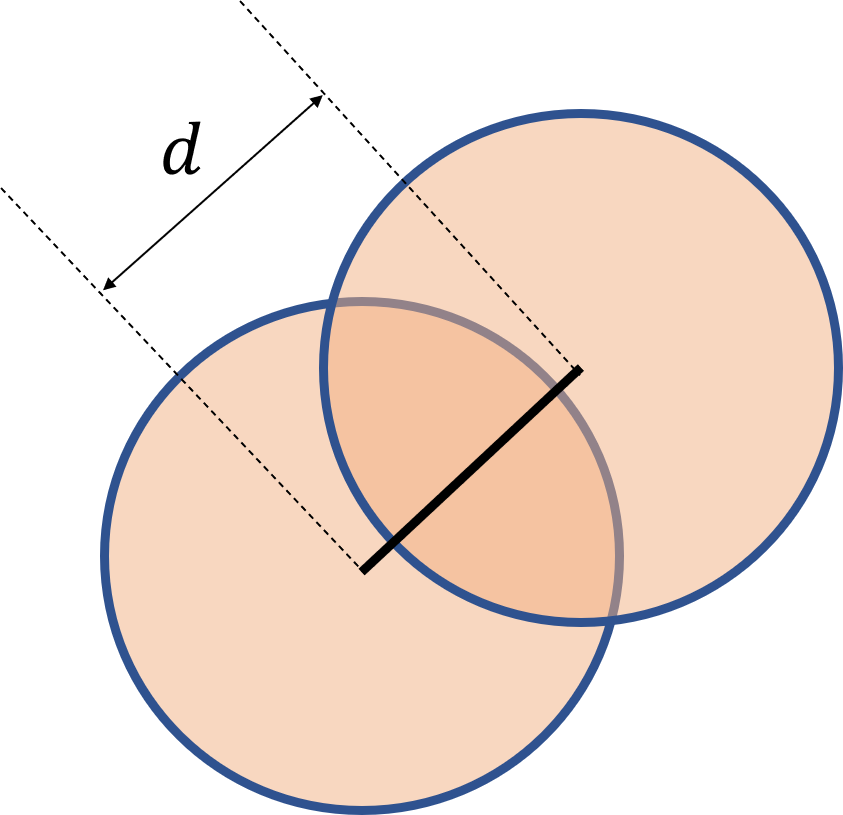
\includegraphics[width=0.7\linewidth, clip]{./figure/merge_circle.png}
    \caption{2台のLiDARが認識した人物の円}
    \label{fig:circle}
\end{figure}

LiDARが認識した人物を示す2円の中心の距離を$d$と置き,1つの円とみなす円の中心距離の最大値を$d_{max}$とすると
$d < d_{max}$のときに2つの円は同一人物を認識していると見なし1つの円に統合する.


\subsection{オクルージョンが発生した場合の撮影計画の補完}
LiDARの設置位置と人物の位置関係からLiDARが物体を認識することのできない領域を推定することができる.
この領域をオクルージョンエリアと定義する.オクルージョンエリアは人物の円に対してLiDARの座標を通る2本の接線を考え,
2接点を結んだ線と2本の接線,人物の移動可能範囲の境界に囲まれる領域になる.
オクルージョンエリアに撮影ベクトルを付与するために架空の人物(ダミー)を配置することでUAVがその領域を撮影できるようにする.
ダミーの座標の位置は,LiDARと人物を表す円の中心座標を結ぶ直線と人物移動可能範囲の領域との交点を
導出し,その交点の座標と人物の円の中心座標の中点に設定する.
LiDARの座標を$x_{lidar}$,$y_{lidar}$,人物の円の中心座標を$x_{person}$,$y_{person}$とすると
2点を結ぶ直線の方程式は\cref{eq:occlusion}で求めることができる.\cref{eq:occlusion}の方程式より境界の座標を代入することにより交点の座標が求められる.
1人の人物に対して1つのダミーが生成されるためダミーを含めた人物の数は,
LiDARが認識している人物の数を$n$人とすると,撮影ベクトルを付与される人物とダミー人物の合計の数は$2n$となる.

\begin{equation}
    \begin{aligned}
       y = \frac{y_{person} - y_{lidar}}{x_{person} - x_{lidar}} x + 
\frac{x_{person}y_{lidar} - x_{lidar}y_{person}}{x_{person} - y_{lidar}}
    \end{aligned}
    \label{eq:occlusion}
\end{equation}


\section{実環境におけるシステム構築}
本研究では,ロボット用のソフトウェアプラットフォームであるRobot OperationSystem(ROS)を利用している.
全体的なシステムは佐々木らが使用していたものとほぼ同じであるが,LiDARの情報を有線でホストPCに送信していたところを
RaspberryPi経由で無線通信に切り替えた.\cref{fig:system}は今回構築したシステムの概略図である.

\begin{figure}[h]
    \centering
    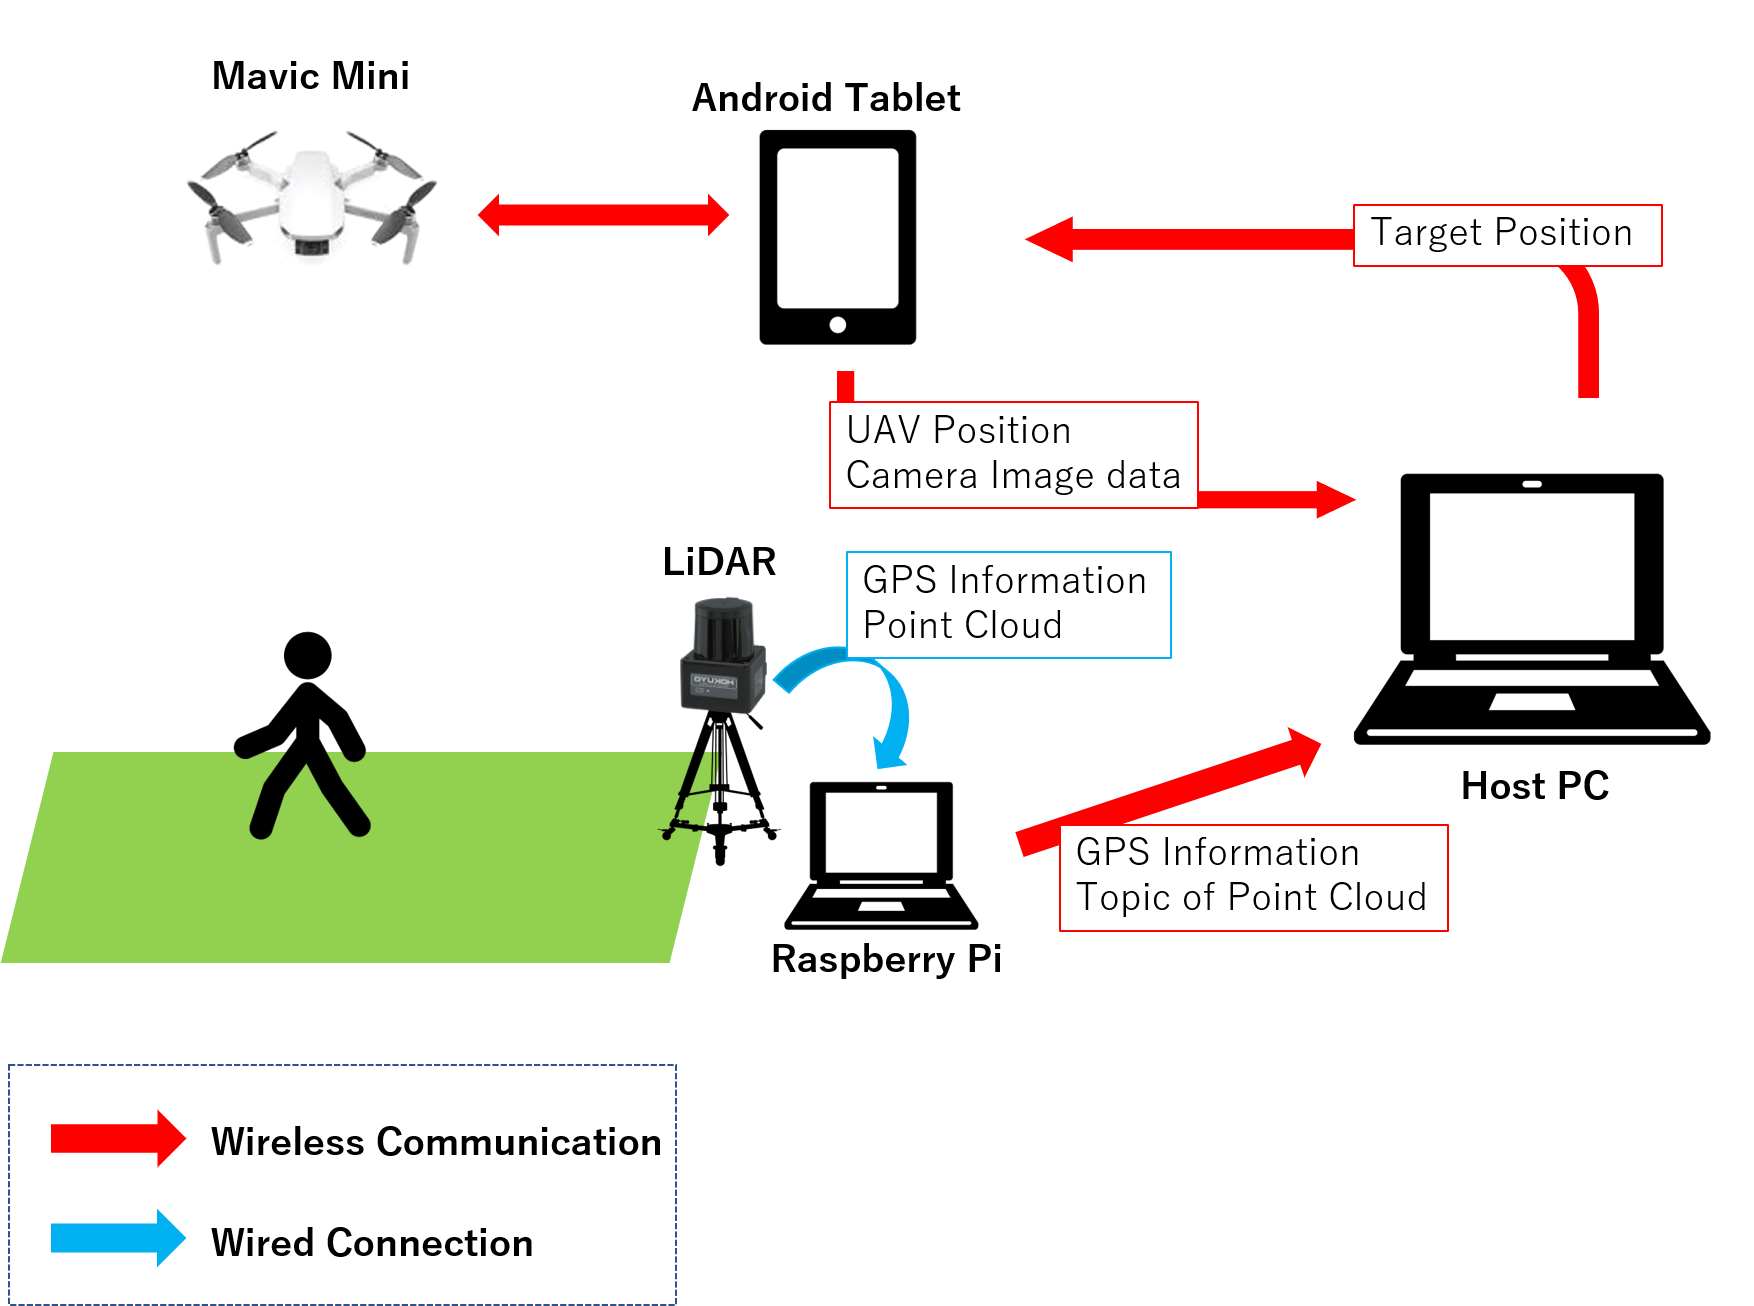
\includegraphics[width=0.7\linewidth, clip]{./figure/communication_model.png}
    \caption{通信モデル}
    \label{fig:system}
\end{figure}


\section{実機実験と考察}
\subsection{ダミーを配置したときの撮影計画}
領域内に2人の人物を配置し同様の動きをした時の撮影計画の比較を行う.

\begin{figure}[h]
    \centering
    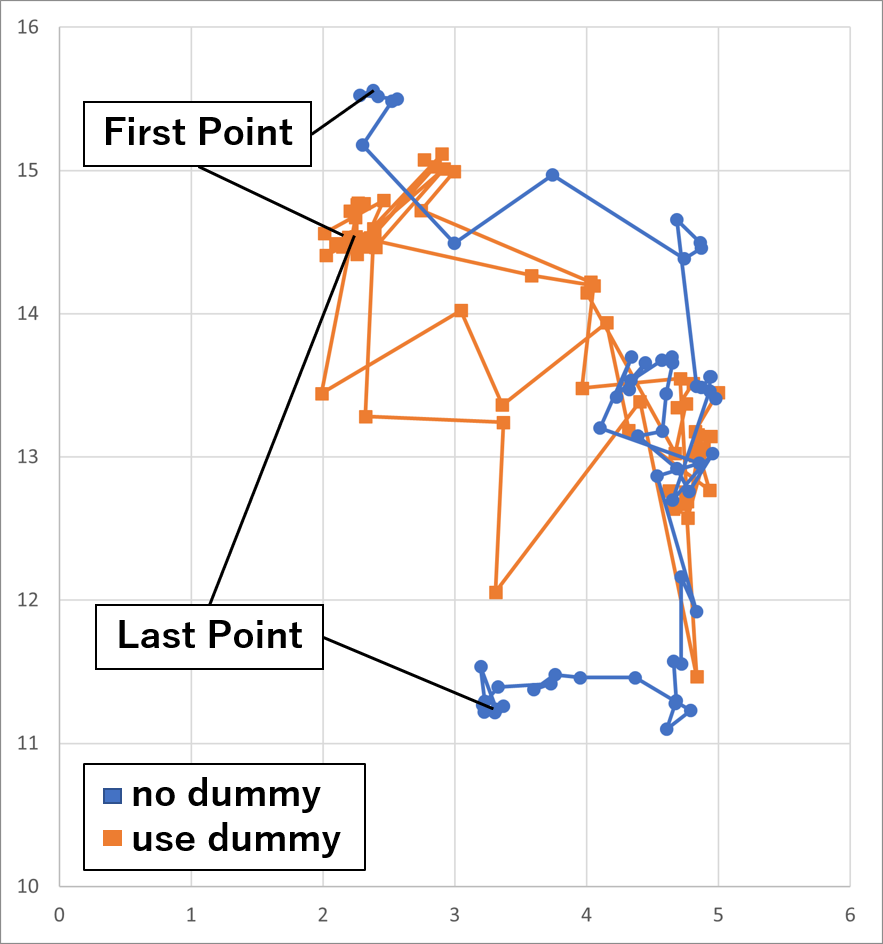
\includegraphics[width=0.7\linewidth, clip]{./figure/goal_graph.png}
    \caption{UAVの目標位置の比較}
    \label{fig:system}
\end{figure}

終点付近を見るとダミーを配置場合はしない場合に比べて北側に目標位置が設定されていることが読み取れる.
ダミーの位置は実際の人物よりも北側に作成されるためそれに伴いUAVの目標位置も北になっていると推測でき,ダミーの配置によりオクルージョンエリアを考慮した撮影計画ができていると考えられる.

\subsection{2台のLiDAR情報の統合の結果と考察}
同一人物を認識した際の情報の統合について考察を行う.
3人の人物を横並びに並べ人物の認識をした結果を画像で示す.

\begin{figure}[h]
    \centering
    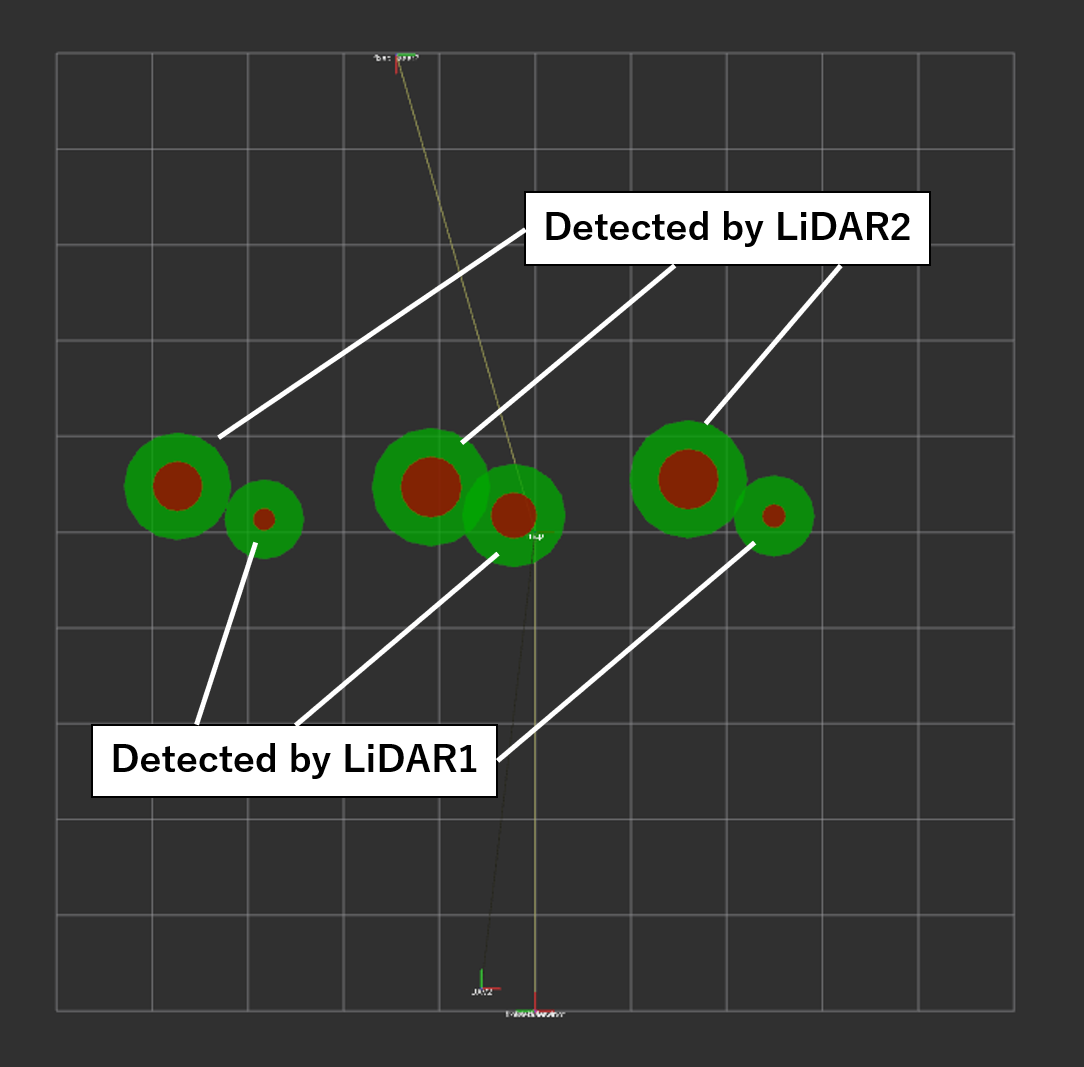
\includegraphics[width=0.7\linewidth, clip]{./figure/row.png}
    \caption{人物3人に対しての各LiDARの認識}
    \label{fig:row}
\end{figure}

1人の人物に対して各LiDARが認識した2つの円が示されている.
この2円の距離は画像左の人物から0.8247, 0.9385, 0.9223であり,$d_{max}$を0.9385[m]にすると全ての人物を表す2円が統合されることになる.人間の横幅を50	cmとすると2人の人物の最短中心間距離は50cm となる.これより$d_{max}$は人間の横幅程度の長さが適切であり0.9385mは誤った統合をしてしまう可能性がある.中心間距離が大きくなった原因としてはLiDARの角度のずれが大きいことがあげられる.LiDARの角度はコンパスを利用して手動で角度を設定しているため誤差が乗る可能性が非常に大きい.

\section{まとめ}
ダミーの配置の実験に関してはオクルージョンを考慮した撮影計画が行えていると推測できる.より効率的に撮影を行うためにオクルージョンエリアに置くダミーの位置や数を調節する必要がある.
LiDARを2台使用する人物認識に関しては,実機実験を行う際の誤差が大きくなるため,角度のキャリブレーション方法を考え直す必要がある.また認識された2つの円のずれと各LiDARの座標からLiDAR同士の角度のずれを算出する手法が提案できる.
今後の展望としては,実験全体で生じる誤差を小さくする設定方法の手法を提案し,複数のLiDARを使用した際に生じるオクルージョンエリアに対するダミーの位置の導出を行い,画像情報と合わせてUAVの撮影計画を最適化することがあげられる.

% bibliography
\begin{thebibliography}{9}

\bibitem{bethke_2007}
Bethke B, Valenti M, and How J, ``Cooperative vision based estimation and tracking using multiple UAVs'', Advances in cooperative control and optimization, pp.179--189, 2007.

\bibitem{bajracharya_2009}
M Bajracharya, B Moghaddam, A Howard, S Brennan, and L H Matthies, ``A Fast Stereo-Based System for Detecting and Tracking Pedestrians from a Moving Vehicle.'', The Int'l J. Robotics Research, Vol.28,pp.1466--1485, 2009.

\bibitem{sasaki_2019}
佐々木徹 ``地上設置LiDARと複数UAVを用いた人物追従システムに関する研究'', 大阪市立大学 修士論文,2019
\end{thebibliography}

\end{document}